\documentclass[]{solarphysics}

\usepackage[hyperref,optionalrh,showbiblabels]{spr-sola-addons} % For Solar Physics 

\usepackage{graphicx}        % For eps figures, newer & more powerfull
\usepackage{amssymb}        % useful mathematical symbols
\usepackage{color}           % For color text: \color command
%\usepackage{breakurl}        % For breaking URLs easily trough lines
\def\UrlFont{\sf}            % define the fonts for the URLs

\usepackage{natbib}
\bibliographystyle{spr-mp-sola}


%Journal commands from AAStex
\newcommand\procspie{\ref@jnl{Proc.~SPIE}}%      % Proceedings of the SPIE 
\newcommand\apj{\ref@jnl{ApJ}}%    % Astrophysical Journal 
\newcommand\apjl{\ref@jnl{ApJL}}     % Astrophysical Journal, Letters 
\newcommand\apjs{\ref@jnl{ApJS}}%    % Astrophysical Journal, Supplement 




\begin{document}
\begin{article}
\begin{opening}

\title{Determining the Spectral Content of MOSES Images}

\author[addressref={aff1},corref,email={jacob.parker3@montana.edu}]{\inits{J.D.}\fnm{Jacob D.}~\lnm{Parker}}%\sep
\author[addressref=aff1,email={Want to include your email Charles?}]{\inits{C.C.}\fnm{Charles C.}~\lnm{Kankelborg}}%\sep
\address[id=aff1]{Montana State University}


\begin{abstract}
Abstract last ...
\end{abstract}
\keywords{Need to look through the list of allowed keywords and pick a couple}
\end{opening}

\section{Introduction}
%Cosie as possible broad scientific context

	
	
	Cite successful studies using similar data, including previous MOSES studies. \\ 
	
	Short comings of narrow band EUV imagers.  AIA temperature function for 304 \AA \ image?.  MOSES I throughput curve. \\
	
	Identifying solar features in the MOSES data that have undergone spectral dispersion is simple. Subtracting the central order image (that contains no spectral dispersion) from either outboard order eliminates non-dispersed features. What remains are bi-polar features of various spatial scales.  A feature in the principle wavelength, He {\sc ii} $\lambda 303.8$\AA, with a nonzero line-of-sight (LOS) velocity is translated along image rows.    MOSES has a spectral dispersion of $\approx 30$ km s$^{-1}$ pixel$^{-1}$, leading to a less than ten pixel shift for even the fastest LOS velocities in He {\sc ii}. 
	%It would be nice to nail just need to dig up some grating specs.%
	This results in a bi-polar feature with an obvious positive and negative counterpart that are immediately next to one another. A great example of this is the explosive event studied by \citet{Fox2010} which is highlighted in Figure \ref{}.
	
	Features from other emission lines in the MOSES passband have shifts larger than 10 pixels and cannot be mistaken as Doppler shifted features in He II $\lambda303.8$ \AA. A feature in Si XI $\lambda$303.3\AA , the next closest line, would be shifted by 17 pixels. Si XI features can be seen on the solar limb where He II has little to no contribution. The active regions observed by MOSES have a complicated structure in the difference images.  The northern of the two active regions shows small bi-polar features with positive and negative lobes immediately next to one another.  It also shows a large curved negative feature with no obvious positive counterpart.  We will refer to this feature as the ``wishbone".  The wishbone has a spatial size of \textbf{find this number exactly}.  Therefore its positive and negative parts should appear next to one another if it is shifted by its size or less.  Since this is not the case we can infer that its wavelength is at least \textbf{so many angstroms} different.  Since the wishbone's positive lobe cannot be identified by eye we turn to cross correlation to identify its spectral content.
	

	
	
	

\section{Methods}
	\subsection{Temporary Outline}
		I am having trouble organizing my thoughts for this section.  Lets try this way.
		\begin{enumerate}
			\item Summary
			\item Time Averaged Difference Images
				\begin{enumerate}
					\item Representative Data Set (Not interested in temporal behavior)
					\item Stack Images to increase SNR.
					\item Fill in Saturated Regions
					\item Difference Images quickly reveal spectrally interesting features
				\end{enumerate}
			
			\item Cross Correlation
				\begin{enumerate}
					\item Cross Correlation Equations (Mean as a function of lag)
					\item Why Difference Images
					\item Show Cross-Correlation Function
				\end{enumerate}
			
			\item Significance Testing
				\begin{enumerate}
					\item Looking for Significant Peaks in Correlation
					\item Columns (No Spectral Dispersion)
					\item Building Longer Columns in Fourier Space
					\item Phase Shuffling for Random Data
					\item Correlation Length for Degrees of Freedom
				\end{enumerate}
			
			\item Forward Model
				\begin{enumerate}
					\item Synthetic MOSES images for different DEMs
					\item Coaligned EIT Images
					\item Chianti Temperature Image Selection and Intensity
					\item MOSES PSF Convolution
					\item Linear Combination and Least Squares Minimization with MCMC
				\end{enumerate}
		\end{enumerate}
	

	
 		
 	\subsection{Time Averaged Difference Images}	
 	
 	During its flight on February 8th, 2006 MOSES captured 27 images with exposure times ranging from one to thirty seconds. While MOSES did capture events with interesting temporal behavior \citep{Fox2010,Rust2017} our study aimed to quantify the total observed spectral content. Therefore we preformed our analysis on a time averaged version of the data.
 	
 	Longer exposures are best for observing quiet sun features but are saturated near active regions.  To fill in missing saturated regions and increase signal to noise we form a single time averaged image in all three spectral orders. Saturated pixels are masked with NaNs (Not a Number) and treated as missing data. Since MOSES observes through changing amounts of atmosphere throughout its flight we use the median of each image as a synthetic exposure time, rather than the amount of time the shutter is open.  %Actually you wouldn't want to ignore saturated pixels when taking the median.  All that matters is that those pixels are a high value and, unlike the mean, those values are irrelevant. Check and see how you did this.
 	Masked data is then summed in time and divided by a total exposure time for each pixel to form a single time averaged image in each spectral order with no saturated pixels.  Figures \ref{fig:moses_super}a and \ref{fig:moses_super}b shows the m = 0 and 1 order time averaged images. 
 	
 	\begin{figure}
 		\begin{center}
 		\begin{tabular}{lll}
 			\begin{minipage}{.29\columnwidth}
 				\resizebox{1\columnwidth}{!}{\includegraphics{super_zero}}
 				
 			\end{minipage}&
 			\begin{minipage}{.29\columnwidth}
 				\resizebox{1\columnwidth}{!}{\includegraphics{super_plus}}
 			 
 			\end{minipage}&
 			\begin{minipage}{.29\columnwidth}
 				\resizebox{1\columnwidth}{!}{\includegraphics{super_pz}}
 		
 				
 			\end{minipage}
 		\end{tabular}
 		\end{center}
 		\caption{Figure of MOSES super exposures and a difference image}
 		\label{fig:moses_super}
 	
 	\end{figure}
 	
 	 The difference between two spectral orders reveals several interesting features.  Figure \ref{fig:moses_super}c shows many small bipolar features throughout the quiet sun and a few large features in active regions and near the limb that are boxed in green.  The northern most green box has a large, coherent, negative feature dubbed the ``wishbone''.  The wishbone is very solar in appearance (possibly a partially filled active region loop), and has no obvious positive counterpart.  Close inspection reveals a white smear to its left that is likely a shifted wishbone in the plus order.  Unfortunately the positive portion of the wishbone is too blurry to quantify its shift by inspection.  In order to quantify subtle differences between orders we turn to cross-correlation.
 	
 	
 	\subsection{Cross-Correlation}
 	
 	 	
 	 	\begin{figure}
 	 		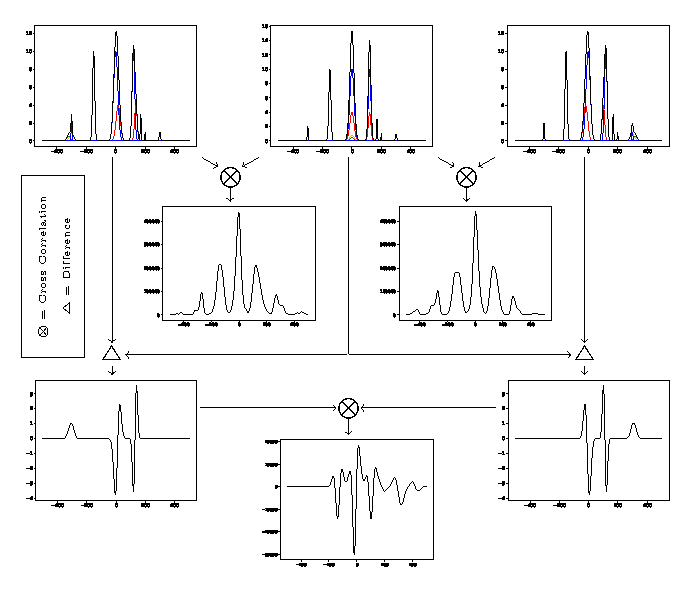
\includegraphics[scale = 1]{methods_fig.pdf}
 	 		\caption{A graphical representation of our cross-correlation procedure}
 	 		\label{fig:methods}
 	 	\end{figure}
	
 	To help identify subtle pattern repetition in the MOSES difference images we cross-correlated them along the dispersion direction, or image rows.  The cross-correlation of two difference images is defined to be,
	 	\begin{equation}
		 	PZ \otimes MZ = \mathcal{F}^{-1} \left\{\mathcal{F}\left(PZ \right)*\mathcal{F}\left(MZ \right)  \right\},
		 	\label{eqn:cross_correlate}
	 	\end{equation}
 	where $PZ$ and $MZ$ are the m = 0 order subtracted from the m = 1 order and the m = 0 order subtracted from the m = -1 order respectively. $\mathcal{F}$ is the Fast Fourier Transform (FFT) operator.  The MOSES image rows were also Hanning windowed prior to applying the FFT to minimize edge effects.  The discrete Hanning window, $w(k)$, implemented was,
 	
		\begin{equation}
			w(k) = \alpha - (1-\alpha)\mathrm{cos}\left( \frac{2\pi k}{N} \right) \ \mathrm{for} \ k = 0,1,...,N-1 \quad ,
			\label{eqn:Hanning}
		\end{equation}
	where $N$ is the number of elements in the array being windowed and $\alpha = .5$.
 	
 	Preforming a cross-correlation on the difference images requires justification.  An obvious first choice would have been to simply cross-correlate the m = 0 order with either outboard order.  Unfortunately the correlation function is dominated by the autocorrelation of the He {\sc ii} signal as seen in Figure \ref{fig:methods}(put a letter here).  This would also be the case when cross-correlating the m = 1 and m = -1 order images.  By taking the difference we remove stationary He {\sc ii} objects from the images and in turn their autocorrelation from the cross-correlation functions.
 	
			 	
		\begin{figure}
		\centering
		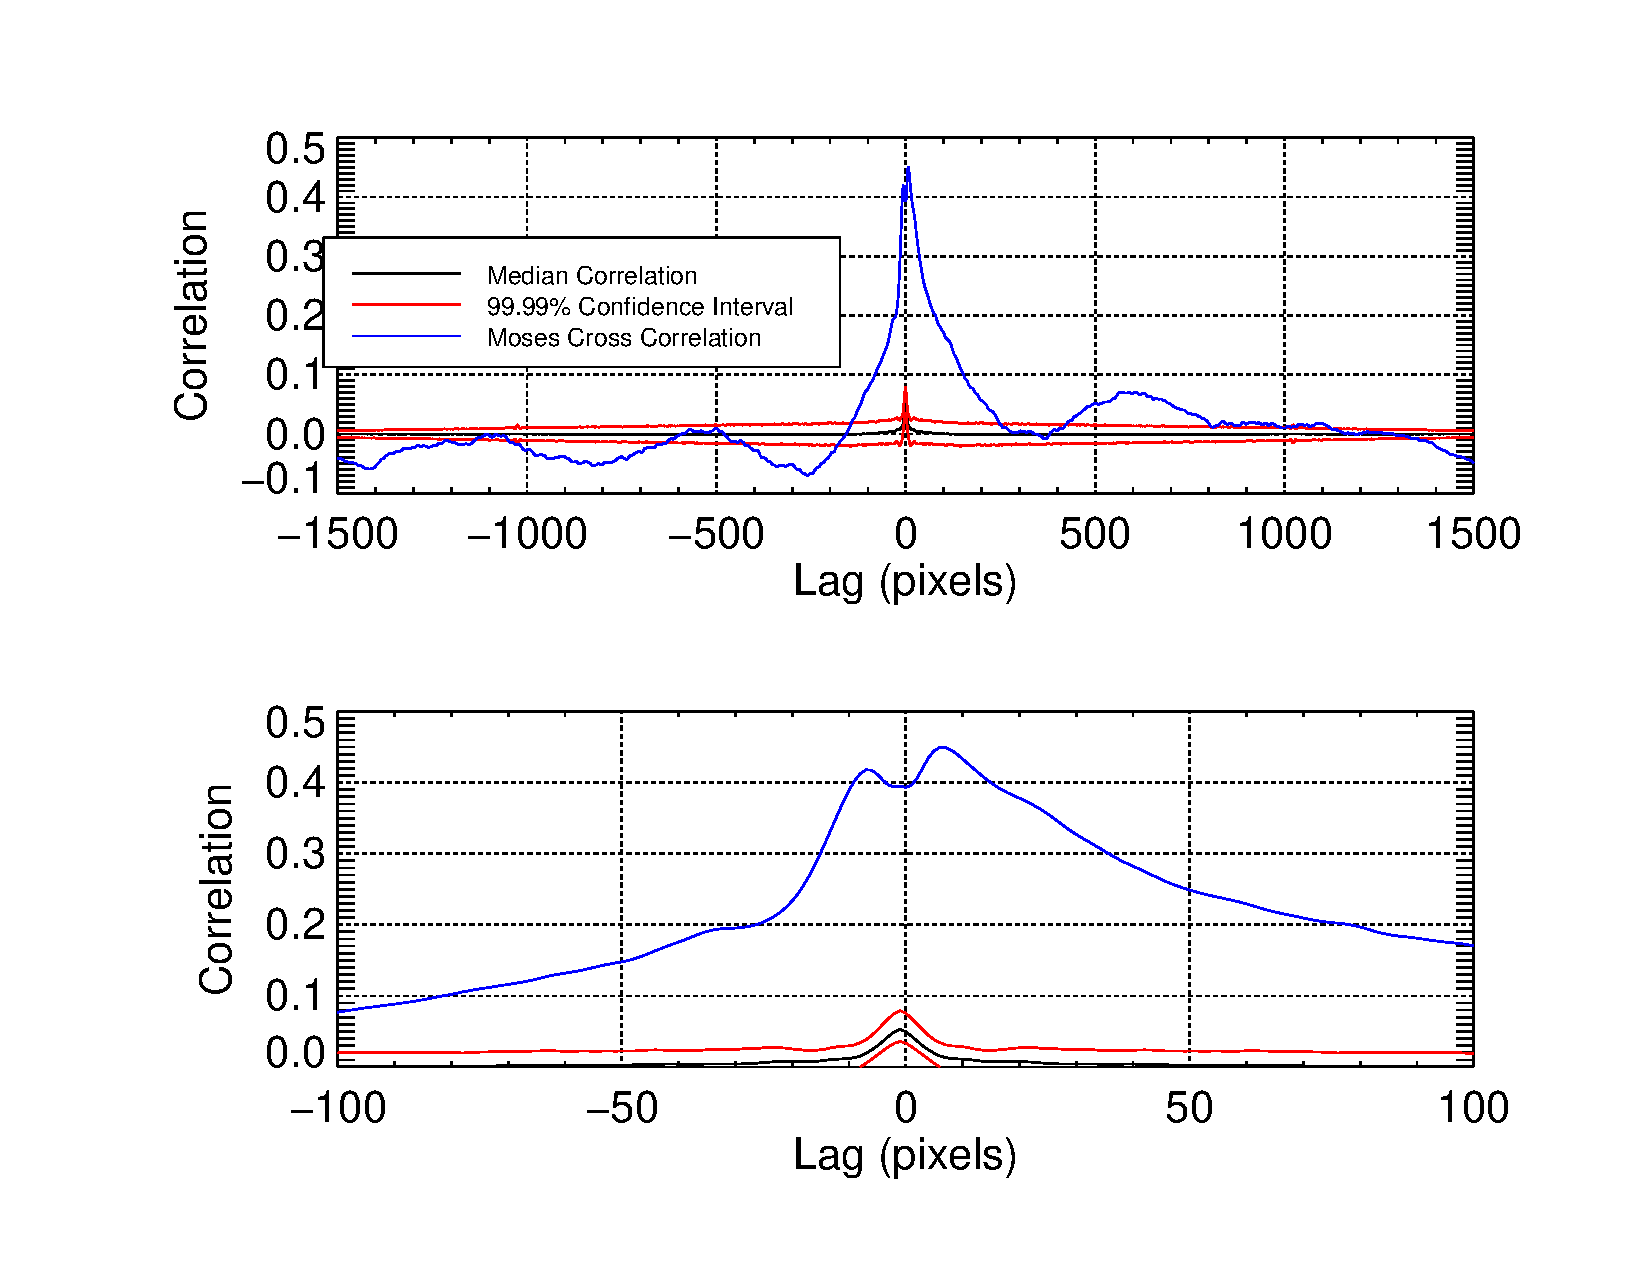
\includegraphics[width=\linewidth]{images/sigtest_5}
		\caption{The mean cross-correlation function of MOSES difference image rows (blue) overlaid on the 99.99 percent confidence interval formed by cross-correlating random data (red). }
		\label{fig:sigtest}
		\end{figure}
 	
	 This procedure yields a one dimensional cross-correlation function for each row of the MOSES difference images.  Since we are concerned mostly with bulk spectral content we then take the mean of all 1024 cross-correlation functions, one for each row, to get our final correlation curve plotted in blue in Figure \ref{fig:sigtest}. 
	 
	 The cross-correlation curve or the MOSES difference images has a few notable features.  There are several noticeable peaks in correlation  at approximately $-800$, 250, and 600 pixel lags.  The largest peak in correlation, centered about zero lag, also displays a double peak, not typical of auto-correlation functions that generally have  maxima at zero lag for uncorrelated functions.  While these features are identifiable, the curve is complicated enough that quantifying peaks in correlation visually is difficult and the significance of any given peak is questionable. We therefore move to test the null hypothesis that none of these features are statistically significant by cross-correlating random data generated to match the MOSES image rows.
 
	
	\subsection{Significance Testing}
	\label{sec:sigtesting}
	The mean cross-correlation function of the two MOSES difference images, $PZ$ and $MZ$, has several peaks at nonzero lags.  We propose that these peaks in cross-correlation are due to shifted solar features in the MOSES outboard orders and are therefore significant in identifying extra spectral content.  To test this hypothesis we cross correlated randomly generated synthetic solar data that matched MOSES image rows in length and had similar power spectral and autocorrelation distributions.  Our test data set was generated from the MOSES image columns because they contain the same solar features as the image rows, but contain practically no spectral dispersion.  By interpolating and shuffling the elements of the MOSES columns in Fourier space we can generate a large number of test arrays for significance testing.
	
	MOSES images contain 2048 columns.  These columns have the same spatial features as MOSES image rows but with none of the spectral information.  Despite this the MOSES image columns are insufficient for significance testing in a couple ways.  First, there is an insufficient sample size.  With features in the MOSES images ranging from four to about a hundred pixels we have at most 512 unique columns for significance testing.  Second, they are half as long as the rows preventing us from measuring significance past 1024 pixel lag.  Therefore we needed to generate a synthetic data set for significance testing.
	
	Using the MOSES image columns as our basis we generated $N$ random arrays that are 2048 long and match MOSES columns in both power spectral and autocorrelation distribution.  First the columns in each image, $P(x,y)$, $Z(x,y)$, and $M(x,y)$, are windowed with a Hanning window, $w(y)$(Equation \ref{eqn:Hanning}), and Fourier transformed along the column dimension, $y$.  The windowed Fourier transformed array is defined to be
	
	\begin{equation}
		\widetilde{Z}_w[x,k] = \mathcal{F}_y\left[ w(y)Z[x,y]\right], 
		\label{eqn:ztwiddle}
	\end{equation}
	where, $ x = 0,1,...,2047$ and $y = 0,1,...,1023$.  In Equation \ref{eqn:ztwiddle} and the following equations we will show the procedure used to generate random arrays for only the zero order, $Z(x,y)$, for simplicity even though an identical procedure was carried out on every order.
	
	The transformation outlined in Equation \ref{eqn:ztwiddle} gives us 511 spatial frequency bins and one DC bin that each have 1024 elements, one for each column, for each order.  Each new array, $\widetilde{Z}^{'}$, is formed by picking an element randomly from each frequency bin. To further scramble the array each value of $k$, aside from the DC term, is given a random phase shift, $e^{i\phi}$.  By this method the $k^{\mathrm{th}}$ element in each new synthetic array, $\widetilde{Z}_k^{'}$, is found as follows:
	
	\begin{equation}
		\widetilde{Z}_k^{'} = \widetilde{Z}_w\left[\sigma(m,2048), k  \right]e^{i\Phi(n)} ,
		\label{eqn:synth_array}
	\end{equation}
	where,
	
	\begin{equation}
		\sigma(m,L) = floor\{randomu(m)*L\} ,
	\end{equation}
	\begin{equation}
		\Phi(n) = 2\pi * randomu(n),
	\end{equation}
	the function $randomu()$ picks a random value from a uniform distribution between zero and one each time it is called, and $floor()$ rounds down to the nearest integer.  The function $\sigma()$ generates a random integer between zero and $L-1$.  
	
	In order create an array that is 2048 elements long from one that is 1024 elements long we require twice as many value of $k$.  We solve this problem by double picking values from the distribution for each wave number, $k$.  The values of $k$ used in Equation \ref{eqn:synth_array} are,
	
	\begin{equation}
		k_j = floor(j/2),
	\end{equation}
	where $j = 1,2,..,1022.$ Since our data is purely real we can fill in the remaining Fourier components,  negative frequencies, with the complex conjugate of the corresponding positive frequency component.  The final synthetic MOSES row is found through a FFT, 
	
	\begin{equation}
		Z^{'} = \mathcal{F}_y^{-1}[\widetilde{Z}^{'}].
	\end{equation}

	To verify that our N synthetic arrays match the MOSES columns we take a 1024 element long section of each synthetic array, as well as the MOSES columns, and plot portions the power spectral and autocorrelation distributions. Figures \ref{fig:sigtestpower} and \ref{fig:sigtestauto}  show three percentiles of the distribution (10th, 50th, and 90th) for both power spectra and autocorrelation for N equal to 10,000 synthetic arrays. Figure \ref{fig:sigtestpower} shows great agreement between synthetic data and the MOSES columns in power spectral distribution.  Figure \ref{fig:sigtestauto} show good agreement between the synthetic data and MOSES columns at the median and only marginal agreement in the wings of the distribution.  Despite that the synthetic data always has a high autocorrelation length that the MOSES columns and therefore acts as a worse case scenario during significance testing.  
		
	\begin{figure}
		\centering
		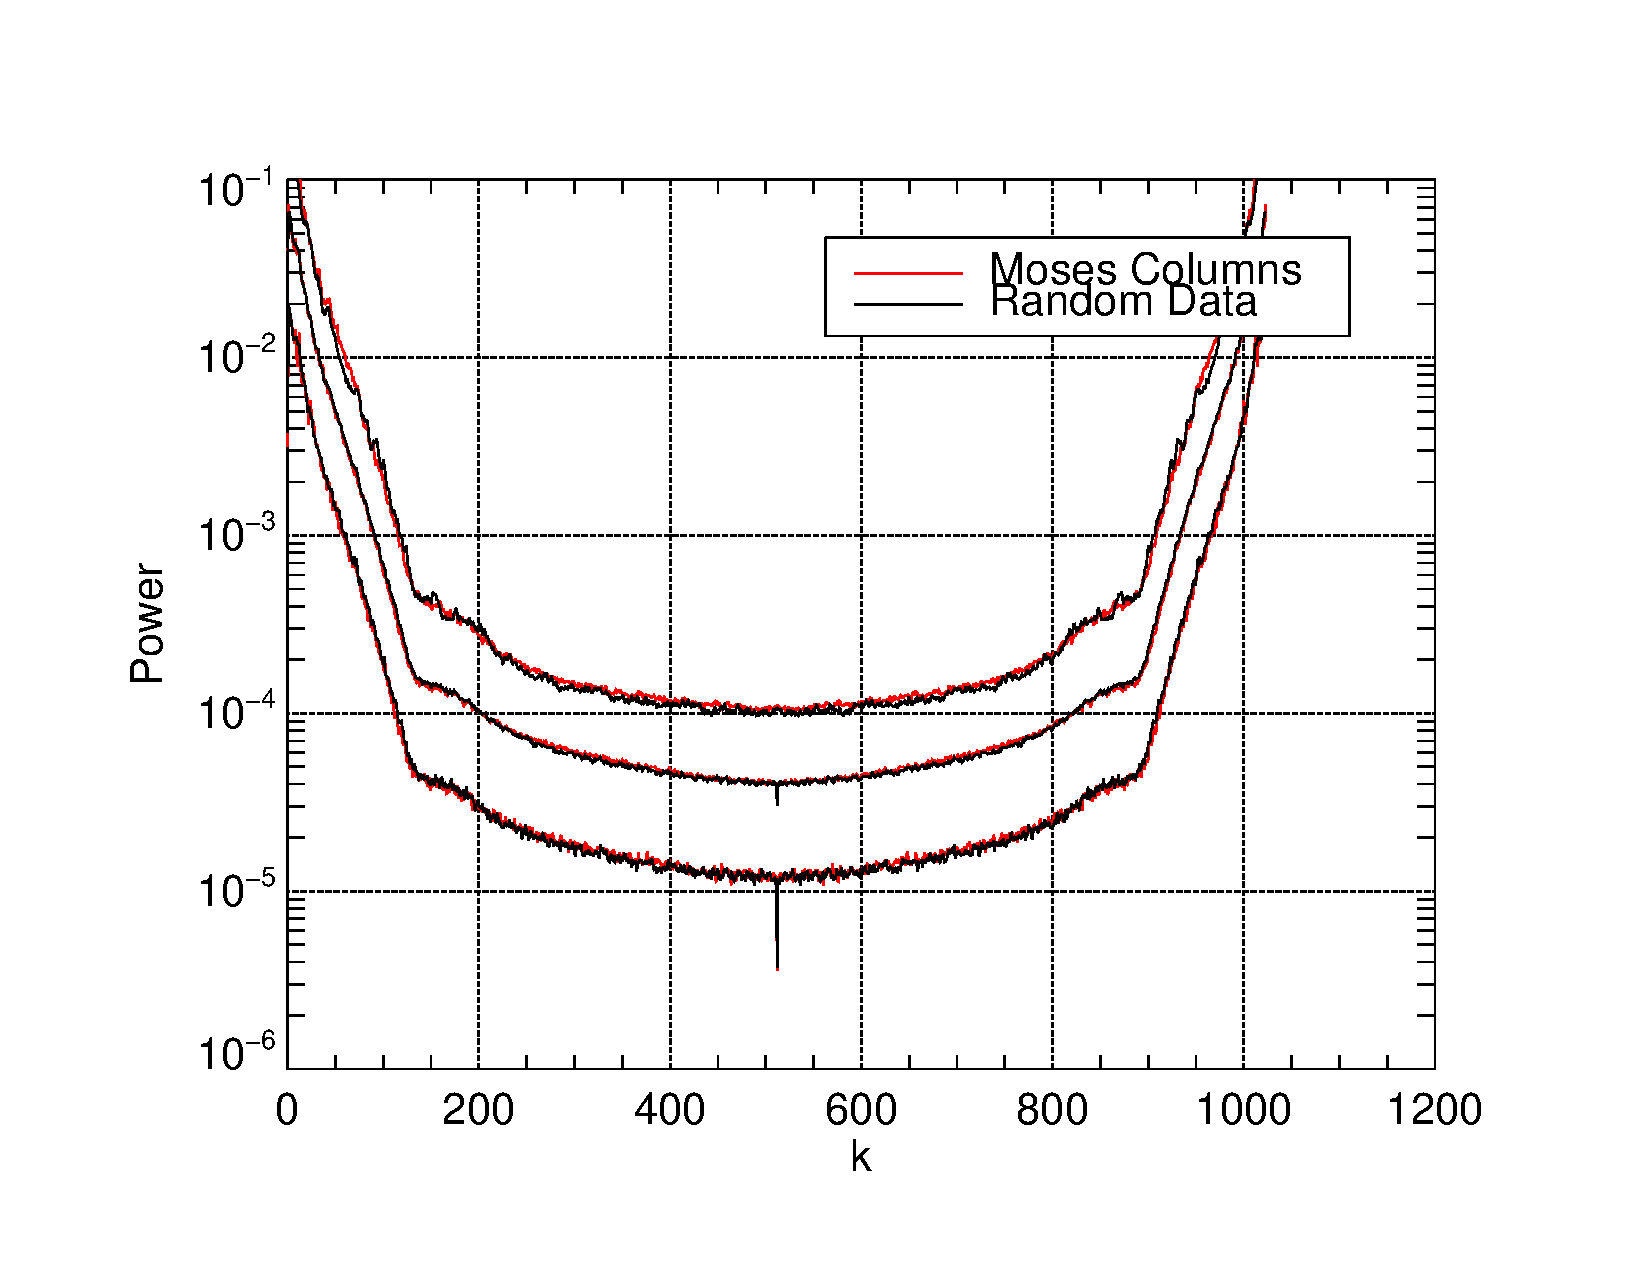
\includegraphics[width=\linewidth]{images/sigtestpower}
		\caption{The 10th, 50th, and 90th percentile of the power spectral distribution for each value of k is plotted for both the MOSES columns and synthetic data.}
		\label{fig:sigtestpower}
	\end{figure}
	\begin{figure}
		\centering
		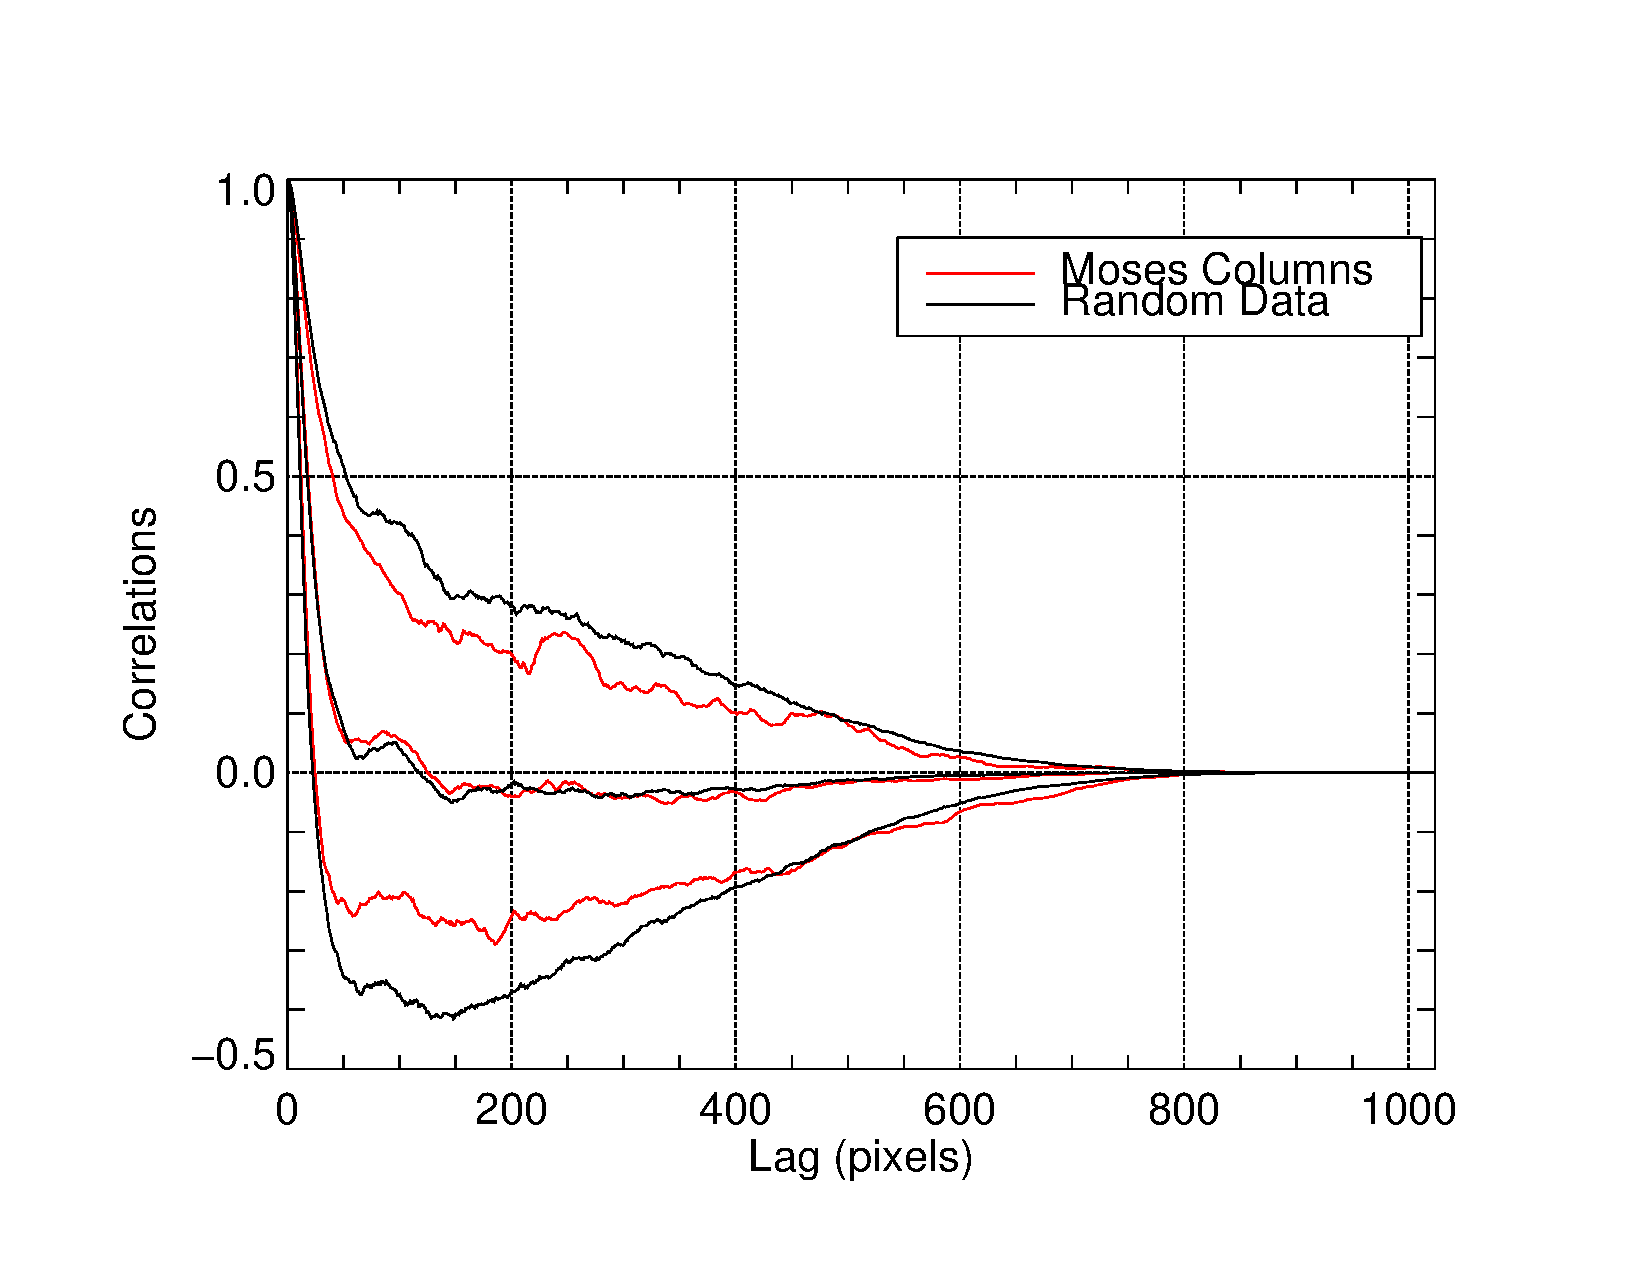
\includegraphics[width=\linewidth]{images/sigtestauto}
		\caption{The 10th, 50th, and 90th percentile of the autocorrelation distribution for each value of k is plotted for both the MOSES columns and synthetic data.}
		\label{fig:sigtestauto}
	\end{figure}
	
	Figure \ref{fig:sigtest} shows the results of our significance testing with 10,000 synthetic arrays.  Each set of three arrays, $Z^{'}$, $M^{'}$ and $P^{'}$, are subtracted and correlated according to Equation \ref{eqn:cross_correlate}. We find that the mean cross-correlation of MOSES difference images along their rows has peaks that are much greater than the 99.99\% confidence interval and are therefore significant and indicative of extra spectral content.
	
	
	
	
	
	\subsection{Forward Model} 
	The mean cross-correlation of MOSES difference image rows is shown in Figure \ref{fig:sigtest}.  In Section \ref{sec:sigtesting} several peaks in correlation were deemed to be significant and indicative of extra spectral content in the MOSES images.  These peaks have irregular, broad profiles and are both positive and negative.  To interpret how these peaks in correlation relate to spectral content we developed a forward model that produces synthetic MOSES difference images with known spectral content using Chianti \citep{} and images from EIT \citep{}.  
	
	During the 2008 MOSES rocket flight EIT captured 4 full disk EUV images, one in each of the 171 {\AA}, 195 {\AA}, 284 {\AA}, and 304 {\AA} channels.  Each image was co-aligned, cropped, and rebinned 
	
	\subsection{Fitting}
	Using a MCMC to thoroughly explore the parameter space and generate error bars on fit parameters. More work to be done here.

\section{Results}
	Synthetic images of best fit.  Quantify extra spectral content.  Comment on extra He II emission unaccounted for by Chianti. 

\section{Discussions/Conclusions}
	Implications for future, design changes incorporated in ESIS (field stop, line selection, dispersion increase?). Possibly examine the spectra surrounding Ne VII 465 \AA.  Do we have the MOSES II throughput curves? 
	
\bibliography{ParkerKankelborg2018}


\end{article}
\end{document}
	
